\chapter{Git}\label{cha:git}
In diesem Kapitel werden auf die wesentlichsten Grundlagen und Befehle
beschrieben, um mit Git Dateien zu verwalten. Als Erstes wird mit einfachen
Befehlen ein Git-Repository erstellt und später am Beispiel dieses Repositorys,
auf weitere Eigenschaften und Befehle eingegangen.

\section{Grundlagen}\label{gitbasics}
In diesem Beispiel werden wir ein Repository \textit{git-example} mit einem
Skript (\texttt{git-stats}) erstellen welches ein paar einfache Statistiken
über die Autoren eines git Repositorys erzeugt.

Alle Beispiele werden auf einer Linux Kommandozeile durchgeführt. Git ist für
alle gängigen Linux Derivate verfügbar. Die Autoren von \cite[S.~12-14]{progit}
gehen auf weitere Details zur Installation von Git in anderen Versionen oder
auf anderen Betriebssystemen ein.

Die in den Beispielen eingesetzte Version von Git ist 2.15.0. Der folgende
Abschnitt basiert zum Zeil auf den Ausführungen der Autoren aus
\cite[S.22-57]{gitosp}

\lstinputlisting[
  label=lst:gitversion,
  caption={Version von Git ausgeben},
  captionpos=none,
]{listings/git_version.lst}

\subsection{Konfiguration}\label{gitconfig}
Zu Beginn sollten einige grundlegende Konfigurationen vorgenommen werden. So
sollten, damit die Nachvollziehbarkeit gewährleistet ist als erstes immer der
Name und die Mailadresse des Benutzers konfiguriert werden. Auch ist die
farbliche Darstellung der Ausgaben durchaus hilfreich. Hier kann Git so
konfiguriert werden, dass die Farbausgabe automatisch unterdrückt wird sollte
die Ausgabe in eine Datei umgeleitet werden.

\lstinputlisting[
  label=lst:gitinitconfig,
  caption={Erste Git Konfiguration},
  captionpos=none,
]{listings/git_init_config.lst}

Die \textit{global} eingestellten Optionen können ebenfalls direkt in der Datei
\texttt{\textasciitilde/.gitconfig} eingesehen und bearbeitet werden.
Zusätzlich können für jedes Repository spezifische Konfigurationen vorgenommen
werden. Hierzu muss der Parameter \texttt{--global} bei dem o.a. Befehl
entfernt werden. Die zugehörige Konfigurationsdatei findet sich in jedem
Repository unter dem Pfad \texttt{.git/config}.

\subsection{Erstellen eines Repositorys}\label{startup}
Damit Dateien nun mit Git versioniert werden können, muss wie folgt ein
(lokales) \gls{repository} erstellt werden:

\lstinputlisting[
  label=lst:gitinit,
  caption={Repository anlegen},
  captionpos=none,
]{listings/git_init.lst}

Sollte das Verzeichnis \texttt{hello\_seminar.git} noch nicht existieren, wird
es angelegt. Zusätzlich wird innerhalb von \texttt{hello\_seminar.git} noch ein
weiteres Verzeichnis \texttt{.git} erzeugt, in dem, neben der Konfiguration,
alle Daten abgelegt werden die Git zur weiteren Verwaltung des \glspl{repository}
benötigt.

Um den Status des aktuell erzeugten \glspl{repository} auszugeben kann der
Befehl \texttt{\$ git status} verwendet werden:

\lstinputlisting[
  label=lst:gitstatus,
  caption={Status des Repositorys ausgeben},
  captionpos=none,
]{listings/git_status.lst}

Die von Git erzeugte Ausgabe macht darauf aufmerksam, das noch keine Commits
erzeugt wurden und dass man nun neue Dateien erstellen und hinzufügen kann.

\subsection{Die ersten Commits}\label{sec:first_commits}

Wir werden nun die ersten Dateien zu dem Repository hinzufügen. Dazu laden wir
zwei Dateien mit folgendem Befehl aus dem Internet herunter. Zuvor sollte aber
noch mit folgendem Befehl \texttt{\$ mkdir helpers} ein Unterordner in dem
erzeugten Repository angelegt werden. Wer diese Dateien nicht herunterladen
kann oder möchte, darf selbstverständlich auch einfach Dateien mit gleichem
Namen und beliebigem Inhalt erstellen.

\lstinputlisting[
  label=lst:downloads,
  caption={Herunterladen der Beispieldateien},
  captionpos=none,
]{listings/downloads.lst}

Ab jetzt können die Dateien mit Git verwaltet werden. Ein erstes Hinzufügen
einer Datei mit dem Befehl \texttt{\$ git add LICENSE}, führt zu folgender
Ausgabe von \texttt{\$ git status}:

\lstinputlisting[
  label=lst:add_first_file,
  caption={Eine erste Datei hinzufügen},
  captionpos=none,
]{listings/add_first_file.lst}

Die Ausgabe macht darauf aufmerksam, dass zum Einen, eine neue Datei zum Commit
vorgemerkt ist und zum Anderen, dass sich noch eine Datei im Verzeichnis
befindet, die wir noch nicht mit Git verwalten. Hierbei ist anzumerken, dass
Git auch die vorgemerkte Datei noch nicht wirklich versioniert. Dazu müssen wir
zuerst einen Commit erstellen. Darauf wie Git hier unterscheidet, wird im
Späteren (Abschnitt \ref{sec:trees}) nochmal eingegangen.

Der erste Commit in dem angelegten Repository wird mit dem Befehl \texttt{\$
git commit} erzeugt. Eine Bemerkung zu dem Commit kann, je nach
voreingestelltem Systemeditor jetzt eingegeben werden oder optional mit dem
Parameter \texttt{-m} direkt auf der Kommandozeile übergeben(Listing
\ref{lst:git_first_commit}). In der Bemerkung wird die erste Zeile als Betreff,
und getrennt mit einer Leerzeile alle weiteren Zeilen als ausführliche
Beschreibung verwendet. Dieses Format ist, i.d.R. in den meisten
Versionskontrollsystemen üblich.

\lstinputlisting[
  label=lst:git_first_commit,
  caption={Der erste Commit},
  captionpos=none,
]{listings/git_first_commit.lst}

Darüber hinaus bietet es sich an, sich bem Erstellen solcher Bemerkungen an sich
an gewisse Regeln zu halten. Beispielsweise beschreiben Jez Humble und David
Farley in \cite[S.~37]{cd} eine übliche Situation, bei dem es durchaus sinnvoll
kann, nicht nur zu wissen was der Autor geändert hat, sondern auch warum
und in welchem Kontext. Wenn nicht klar ist, was der Autor sich bei
Änderungen gedacht, hat oder Zusammenhänge nicht aus dem Commit hervorgehen, kann
ein gefundener und behobener Fehler vor dem Veröffentlichen einer
Softwareversion durchaus zu Folgefehlern führen. Solche Situationen enden
nicht selten darin, dass viele Stunden Arbeit investiert werden müssen diese zu
bereinigen.\cite[S.~37]{cd}

Nachdem der erste Commit erzeugt wurde, kann dieser nun mit \texttt{\$ git
show} (Abschnitt \ref{sec:arch}) betrachtet werden. In diesem Fall wurde
beispielhaft eine etwas ausführlichere Bemerkung für den Commit ewählt:

\lstinputlisting[
  label=lst:git_show_first_commit.lst,
  caption={Anzeige des ersten Commits},
  captionpos=none,
]{listings/git_show_first_commit.lst}

Mit \texttt{\$ git show} können alle wichtigen Informationen eines Commits
eingesehen werden.  Neben Zeitpunkt, Autor und Beschreibung auch die
\textit{Commit-ID} (Abschnitt \ref{sec:commit}).  Die weiteren Informationen
werden in einem Format namens \textit{Unified-Diff}\footnote{Details zu dem
\textit{Unified-Diff} Format stellen die Autoren von \textit{GNU diffutils}
unter \cite[S.~12-13]{paper:diffutils} zur Verfügung.} dargestellt, auf welches
hier nicht weiter eingegangen wird.\cite[25]{gitosp}

Wir fügen nun die zweite Datei mit einem weiteren \texttt{\$ git add} hinzu:

\lstinputlisting[
  label=lst:git_add_second_file,
  caption={Eine weitere Datei hinzufügen},
  captionpos=none,
]{listings/git_add_second_file.lst}

Anschließend erzeugen wir einen weiteren \gls{commit} mit:

\lstinputlisting[
  label=lst:commit_git-stats,
  caption={Hinzufügen einer weiteren Datei},
]{listings/commit_git-stats.lst}

Mit diesen beiden zuvor ausgeführten Commits haben wir nun eine, wenn auch
kurze, Historie erstellt. Um diese zu untersuchen dienen die Befehle \texttt{\$
git whatchanged}\footnote{Der Befehl \texttt{\$ git whatchanged} stammt aus
frühen von Git und ist das gleiche wie \texttt{\$ git log} mit einigen
Parametern um die Ausgabe entsprechend zu Formatieren.} oder \texttt{\$ git
log}. Wir werden in Abschnitt \ref{sec:arch} weiter darauf eingehen aber für
diesen Fall ist \texttt{\$ git whatchanged} ausreichend:

\lstinputlisting[
  label=lst:first_git_whatchanged,
  caption={Untersuchen der Historie mit \texttt{whatchanged}},
]{listings/first_git_whatchanged.lst}

Die Ausgabe wird im sogenannten \textit{raw} Format dargestellt. Es werden alle
Commits mit Informationen über den Autor, Commit-ID, Zeit und den veränderten
Dateien in zeitlicher Reihenfolge dargestellt. Die konkreten Veränderungen am
Inhalt der Dateien werden hier nicht dargestellt(Abschnitt \ref{sec:arch} auf
Seite \pageref{sec:arch}).

Erwähnenswert ist noch das Git, im Gegensatz zu anderen
Versionskontrollsystemen, die Dateiberechtigungen speichert. Wer bei den
letzten der beiden Commits auf die Ausgabe geachtet hat (Listing
\ref{lst:commit_git-stats}) dem ist vielleicht folgende Zeile aufgefallen:

\lstinputlisting[
  label=lst:create_mode,
  caption={Create Mode},
  captionpos=none,
]{listings/create_mode.lst}

Diese Ausgabe besagt das es sich hierbei um eine normale Datei handelt (100)
die mit einer, unter Unix üblichen, Berechtigung (664) angelegt ist. Damit
diese Datei aber entsprechend ausführbar ist, müssen wir noch einen weiteren
Commit, mit einer Änderung an den Dateiberechtigungen, erzeugen:

\lstinputlisting[
  label=lst:git_commit_all,
  caption={Commit mit allen Änderungen},
  captionpos=none,
]{listings/git_commit_all.lst}

Mit dem zuvor ausgeführten Befehl haben wir einen Commit erzeugt ohne unsere
Änderungen vorher mit \texttt{\$ git add} hinzuzufügen. Der Parameter
\texttt{-a} bewirkt hier das alle vorhandenen Änderungen zu einem Commit
zusammengefasst werden und nicht einzeln hinzugefügt werden müssen. Zu beachten
ist allerdings das Dateien die Git noch nicht kennt, davon nicht betroffen
sind. Diese müssen nach wie vor zuerst mit einem \texttt{\$git add} hinzugefügt
werden.

Abschließend zu diesem Abschnitt versehen wir den letzten Commit noch mit einer
Markierung bzw. \gls{tag}.

\lstinputlisting[
  label=lst:git_first_tag,
  caption={Anlegen eines Tags},
]{listings/git_first_tag.lst}

Hiermit haben wir einen \gls{tag} mit dem Namen \texttt{tags/0.0.1} angelegt,
der den letzten Commit (\gls{HEAD}) referenziert:

\lstinputlisting[
  label=lst:git_list_first_tag,
  caption={Auflisten von Tags},
]{listings/git_list_first_tag.lst}

Auf den weiteren Umgang mit Tags und welche Arten es gibt wird in den
Abschnitten \ref{sec:managetags} und \ref{sec:tagobject} weiter eingegangen.

\subsection{Verteiltes Git}\label{sec:distributed}
In diesem Abschnitt geht es um die Arbeit mit entferten Repositorys((Abbildung
\ref{fig:centralworkflow})). Die eigentliche Funktionsweise von Git ist, wie
aus Abschnitt \ref{sec:kernel} nochmal deutlicher wird, die verteilte
kollaborative Arbeit an \glspl{repository}.

\begin{figure}[h]
  \centering
  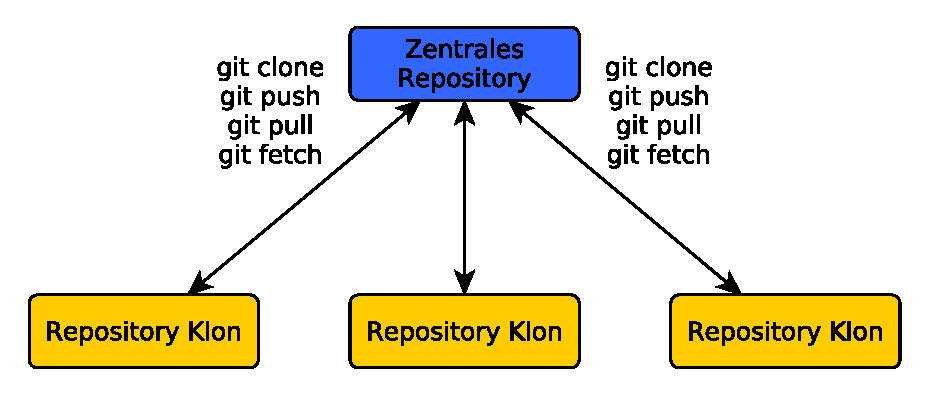
\includegraphics[scale=0.70]{images/workflow.eps}
  \caption{Zentraler Workflow. Angelehnt an \cite[S.~138]{gitosp}}.
  \label{fig:centralworkflow}
\end{figure}

\subsubsection{Erstellen eines Klons}\label{sec:gitclone}
Um eine lokale Kopie eines entferten Repositorys zu erstellen bzw. ein
Repository zu klonen, benötigt man den Befehl \texttt{\$ git clone}. Zum
Transport über das Netzwerk können verschiedene Protokolle benutzt werden.
Unterstützt werden \texttt{ssh,git,http[s],ftp[s]} und \texttt{file}. Eine
entsprechende Url kann neben dem Protokoll noch den Pfad des Repositorys, einen
Benutzernamen oder einen Port enthalten:

\lstinputlisting[
  label=lst:git_url,
  caption={Git Repository-Url },
  captionpos=none,
]{listings/git_url.lst}

Als Besonderheiten gibt es für das Klonen lokaler Repositorys und entfernter
über \acrshort{ssh}, jeweils eine Kurzform. Für das Klonen über \acrshort{ssh} muss das
Protokoll nicht mit angegeben werden und bei lokalen kann vollständig auf die
Angabe einer Adresse verzichtet werden. Hier reicht einfach die Angabe eines
Pfads \texttt{/pfad/zum/repo}.

Das erstellte Beispiel, aus Abschnitt \ref{sec:first_commits}, ist als
Repository verfügbar und kann mit folgendem Befehl geklont werden.

\lstinputlisting[
  label=lst:git_clone,
  caption={Repository klonen},
  captionpos=none,
]{listings/git_clone.lst}

Git speichert die Herkunft des entfernten \glspl{repository} ebenfalls in der
Datei \texttt{.git/config}:

\lstinputlisting[
  label=lst:remote_reference,
  caption={Verfolgtes Repository},
  captionpos=none,
]{listings/remote_reference.lst}

Die gleichen Informationen nur mit Hilfe eines Git Befehl erhält man mit
\texttt{\$ git remote}:

\lstinputlisting[
  label=lst:git_remote,
  caption={Verfolgtes Repository mit \texttt{\$ git remote}},
]{listings/git_remote.lst}

In Listing \ref{lst:git_remote} wird zum einen der Name, in diesem Fall
\textit{origin}, ausgegeben und zum anderen wegen dem Parameter \texttt{-v}
auch der Pfad zum entfernten Repository. Mit \texttt{\$ git remote} können
weitere entfernte Repository, unter anderem Namen, konfiguriert
werden\footnote{Hierzu siehe \texttt{man git remote}}. Ebenso wird
standardmäßig der \gls{branch} \texttt{master} konfiguriert und als sogenannter
\textit{remote-tracking-branch} eingerichtet. Diese Branches sollen die
Änderungen gleichnamiger Branches aus den entfernten \glspl{repository}
verfolgen und werden bei einer Syncronisation automatisch durch Git
aktualisiert.\cite[S.~141-143]{gitosp}

Das weitere Bearbeiten des Repository Inhalts kann wie in dem Abschnitt
\ref{sec:first_commits} beschrieben, durchgeführt werden.

\subsubsection{Änderungen übertragen}
Um Daten in ein entferntes Repository zu übertragen wir der Befehl \texttt{\$
git push} benutzt. Als Standard Ziel wird das Repository verwendet von dem auch
ursprünglich die Kopie erstellt wurde\footnote{I.d.R. ist das \texttt{origin}.}.
initial genutzt wurde, wird weiterhin benutzt.

\lstinputlisting[
  label=lst:git_push,
  caption={Änderungen übertragen},
]{listings/git_push.lst}

In Listing \ref{lst:git_remote} wurde weder der Name des entfernten Repositorys
noch des verwendeten Branches angegeben. In diesen Fall entscheidet Git hier
nach der vorhandenen Konfiguration selbst und ergänzt i.w.S. zu \texttt{\$ git
push origin master}. Wenn der Branch in dem entfernten Repository einen anderen
Namen hat oder ein neuer Branch unter einem anderen Namen angelegt werden soll
kann dieser Vorgang wie in Listing \ref{lst:git_push_other} durchgeführt werden:

\lstinputlisting[
  label=lst:git_push_other,
  caption={Änderungen in einen anderen Branch übertragen},
]{listings/git_push_other.lst}

Mit dem \texttt{push} Befehl können anber auch entfernte Referenzen, wie
Branches oder Tags gelöscht werden. Dazu muss neben dem Namen des entfernten
Repositorys eine leere Referenz mit dem Zielbranch angeben:
werden.\cite[S.~153-155]{gitosp}

\lstinputlisting[
  label=lst:git_push_remove,
  caption={Remote Referenz löschen},
  captionpos=none,
]{listings/git_push_remove.lst}

\subsubsection{Änderungen herunterladen}
Um Änderungen aus entfernten Repositorys herunterzuladen existieren zwei
Befehle. Zum einen \texttt{\$ git push} und zum anderen \texttt{\$ git fetch}.
Der hauptsächliche Unterschied zwischen den beiden Befehlen ist das
\texttt{fetch} lediglich die Änderungen anderer Entwickler aus dem entfernten
Repository herunterläd(Listing \ref{lst:git_fetch}).

\lstinputlisting[
  label=lst:git_fetch,
  caption={Änderungen herunterladen},
]{listings/git_fetch.lst}

Bei dem Befehl \texttt{\$ git pull}, versucht Git nach herunterladen der
Änderungen, diese aus einem entsprechend konfigurierten
\textit{remote-tracking-branch} zu integrieren(Listing \ref{lst:git_fetch}). Der
Befehl ist also eine Kombination aus \texttt{\$ git fetch} und \texttt{\$ git
merge}\footnote{Wenn stattdessen \texttt{\$ git pull --rebase} verwendet wird,
kommt hier eine Kombination von \texttt{\$ git fetch} und \texttt{\$ git
rebase} zum Einsatz. Für weitere Details sei hierzu auf einschlägige
Fachliteratur verwiesen \cite[144-152]{gitosp} oder \cite[85-88]{progit}}.

\lstinputlisting[
  label=lst:git_pull,
  caption={Änderungen herunterladen},
]{listings/git_pull.lst}

\subsection{Objektmodell}\label{sec:objectmodel}
Wie in vorherigen Abschnitten bereits erwähnt, ist das Repository ein
Datenspeicher vergleichbar mit einer Datenbank. Dahinter steht ein Datenmodell
welches sicherstellt, dass die einzelnen Teile eines Commits und deren
Zusammenhänge über die Zeit gewährleistet sind. Dazu verwendet Git ein auf
Objekten basierendes Modell. Dieser Abschnitt geht auf die verschiedenen
Objekttypen und deren Zusammenhänge ein. Er basiert größtenteils auf den
Ausführungen der Autoren aus \cite[S.~49-59]{gitosp}.

Für jedes Objekt wird innerhalb des Repositorys unter \texttt{.git/objects}
eine Datei abgelegt. Für alle Objekte wird eine eindeutige \gls{SHA-1}
Prüfsumme erzeugt, die gleichzeitig als Dateiname und Referenz für das
abgespeicherte Objekt dient. Git unterscheidet zwischen den Objekttypen Tree,
Object, Commit und Tag.

\subsubsection{Trees und Blobs}\label{sec:treeblobobjects}
Zum Speichern von Verzeichnissen verwendet Git ein sogenanntes
\textit{Tree-Object}. Eine Ausgabe der Dateistruktur aus dem verwendeten
Beispiel(Abschnitt \ref{sec:first_commits}) erhält man mit dem Linux Befehl
\texttt{\$ tree}:

\lstinputlisting[
  label=lst:tree.lst,
  caption={Dateibaum des Beispiels},
  captionpos=none,
]{listings/tree.lst}

Um nun den Dateibaum mit der Objektstruktur aus dem Git Repository zur
vergleichen, kann der Befehl \texttt{\$ git ls-tree HEAD} genutzt werden:

\lstinputlisting[
  label=lst:git_ls_tree.lst,
  caption={Objektbaum des Beispiels},
  captionpos=none,
]{listings/git_ls_tree.lst}

Git unterscheidet hier zwischen den angelegten Verzeichnissen und den
eigentlichen Dateien, wie \texttt{helpers/git-stats}. Verzeichnisse werden als
\textit{tree} dargestellt und enhalten, wie auch im Dateisystem, Referenzen auf
weitere Objekte entweder vom Typ \textit{tree} oder \textit{blob}.  Inhalte von
Dateien werden in \textit{blob}-Objekten gespeichert. Allerdings ist der
Dateiname nicht Bestandteil des \textit{blob}, sondern wird in dem
referenzierenden \textit{tree} gespeichert. Dies wird auch nochmal deutlicher,
wenn wir uns das \textit{tree} Objekt zu dem Ordner \texttt{helpers} anschauen:

\lstinputlisting[
  label=lst:git_ls_tree_helpers.lst,
  caption={Objekt eines Ordners},
  captionpos=none,
]{listings/git_ls_tree_helpers.lst}

\begin{figure}[h]
  \centering
  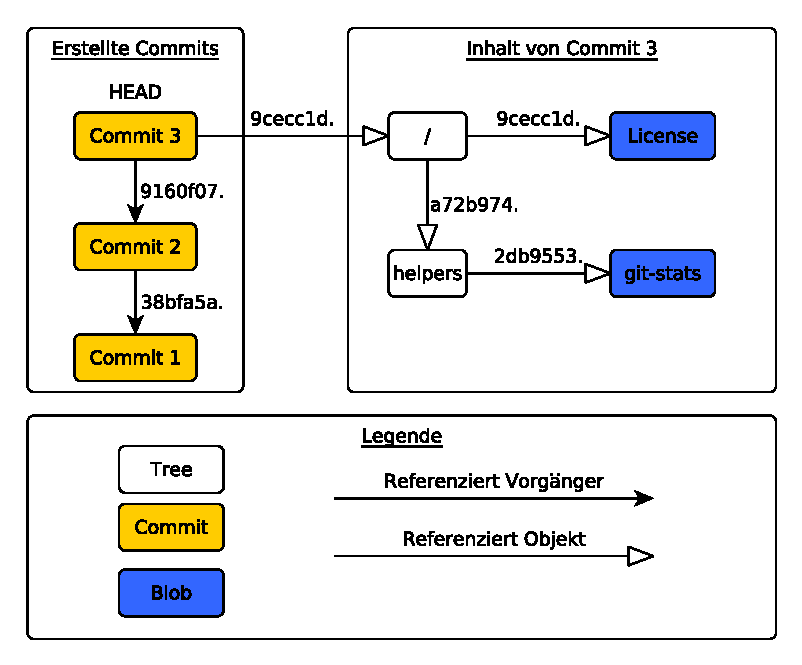
\includegraphics[scale=0.75]{images/objectmodel.eps}
  \caption{Objektmodell zum Beispiel aus Abschnitt \ref{sec:first_commits}.
  Angelehnt an \cite[S.~53]{gitosp}}.
  \label{fig:objectmodel}
\end{figure}

\subsubsection{Commit}\label{sec:commitobject}
Ein Commit-Objekt enthält, neben den bereits bekannten Daten aus Listing
\ref{lst:git_show_first_commit.lst} eine Referenz zu \textbf{einem}
\textit{tree} und ggf. einem vorhergehenden Commit (engl.  \textit{parent}). Im
Fall eines Merge-Commits (Abbildung \ref{fig:merge}) werden enstprechend so
viele Vorgänger referenziert wie branches zusammengeführt wurden. Hier wird
jeweils auf \gls{HEAD} des jeweiligen Branches referenziert. Der in einem
Commit referenzierte \textit{tree} ist, immer ein Verweis auf einen sogenannten
\textit{top-level-tree} (\texttt{/}).  Dieser Verweis referenziert die Wurzel
des entstandenen Objektbaums und enhält keinen Dateinamen(Abbildung
\ref{fig:objectmodel}).

Dadurch das Jeder Commit seinen vorhergehenden Commit referenziert entsteht ein
gerichteter azyklicher Graph bei dem ein Koten durch einen Commit und Kanten
durch Referenzen repräsentiert werden. Ein weiterer Vorteil dieser
Vorgehensweise ist das in dem Commit nicht immer alle enthaltenen Objekte neu
gespeichert werden sondern nur diejenigen die verändert wurden. Alle anderen
referenzieren das ursprünglich angelegte \textit{blob} Objekt. Dieser Effekt
wird als Deduplizierung bezeichnet und führt dazu das ein Repository in dem
eine Datei viele Male existiert bzw. referenziert wird, kaum größer ist als ein
Repository mit nur dieser einen Datei.
\cite[56-57]{gitosp}.

\lstinputlisting[
  label=lst:git_show_raw,
  caption={Ausgabe eines Commits im \textit{raw} Format},
]{listings/git_show_raw.lst}

Zusätzlich unterscheidet Git noch den Committer vom Autor. Diese können sich
unterscheiden wenn Commits z.B. einen Reviewprozess durchlaufen müssen und
nicht von dem Autor selbst in das aktuelle Repository integiert werden(Listing
\ref{lst:git_show_raw}).

\subsubsection{Tag}\label{sec:tagobject}
Ein \gls{tag} markiert einzelne Commits. Hierzu werden i.d.R. Versionsnummern
als Namen verwendet (Abschnitt \ref{sec:tag}). Neben
der \textit{SHA-1-ID} des zu referenzierenden Commits, wird ein Tagname, der
Typ und der Autor (\textit{tagger}) mit Name und Mailadresse gespeichert. Je
nach Art des Tags kann optional noch eine Beschreibung angegeben werden. Bei
Tags ist nicht nur die Prüfsumme, sondern auch der Name eindeutig. Wird
versucht ein Tag mit einem bereits existierenden Namen zu erzeugen, dann
reagiert Git mit einer Fehlermeldung und lehnt das Erstellen entsprechend ab.

Git unterscheidet zwischen drei Arten von Tags:

\begin{enumerate}
\item \textbf{Lightweight Tags:} Dieser Typ ist die einfachste Variante. Er
enthält neben den benötigten Daten wie Autor, Commitreferenz und Prüfsumme
lediglich den Namen. Erzeugt wird er mit dem Befehl:

\lstinputlisting[
  label=lst:git_light_tags,
  caption={Lightweight Tags},
  captionpos=none,
]{listings/git_light_tags.lst}

\item \textbf{Annotated Tags:} Annotated bedeutet nichts Anderes als
kommentiert. Zusätzlich zu den Daten aus den einfachen Tags, wird hier wie bei
einem Commit ein Texteditor geöffnet. Alternativ kann auf der Kommandozeile
ebenfalls mit dem Parameter \texttt{-m} eine Beschreibung übergeben
werden.

\lstinputlisting[
  label=lst:git_annotated_tags,
  caption={Annotated Tags},
  captionpos=none,
]{listings/git_annotated_tags.lst}

\item \textbf{Signierte Tags:} Vorausetzung für diese Art von Tags, ist ein
vorhandener privater \textit{GPG-Key}. Diese Tags werden mit einer Signatur,
versehen die von anderen entsprechend überprüft werden kann, um die Identität
des Autors eindeutig zu verifizieren\footnote{\url{https://gnupg.org}}.
Erstellt werden signierte Tags mit dem zusätzlichen Parameter
\texttt{-s} angelegt:

\lstinputlisting[
  label=lst:git_signatured_tags,
  caption={Signierte Tags},
  captionpos=none,
]{listings/git_signatured_tags.lst}

Zuvor muss Git der zu verwendene Key noch bekannt gemacht werden. Das
kann mit folgendem Befehl erreicht werden:

\lstinputlisting[
  label=lst:git_add_key,
  caption={Signierte Tags},
  captionpos=none,
]{listings/git_add_key.lst}
\end{enumerate}

\subsubsection{Branch}\label{sec:branchobject}
Eine einfache Antwort auf die Frage warum ein Branch nun kein Objekt ist, liefert
das Ausgeben der Referenzdatei des Branches \textit{master}:

\lstinputlisting[
  label=lst:cat_master.lst,
  caption={Referenz \textit{master}},
  captionpos=none,
]{listings/cat_master.lst}

Die ausgegebene Prüfsumme ist in diesem Fall lediglich die \textit{SHA-1-ID} des
letzten Commits aus Abschnitt \ref{sec:first_commits}. Branches sind einfach
Textdateien, die eine Commit-ID zu einem referenzierenden Commit enthalten. Da
diese Referenz veränderbar ist und keine weiteren Informationen enthält, wird
hier kein weiterer Objekttyp benötigt. Da der Name des Branches direkt abhängig
von der erstellten Referenzdatei ist, sind auch die Namen von Branches
eindeutig.

Neben der fortgeschrittenen Manipulation von Git Objekten stellen die Autoren
Scott Chacon und Ben Straub in \cite[S.~408-418]{progit} eine ausführlichere
Sicht auf die Objektverwaltung dar.

\subsection{Bäume}\label{sec:trees}
Git organisiert das Repository in drei verschiedene Bereiche. Scott Chacon,
einer der Autoren von \cite{progit}, spricht in einem seiner
Vorträge\cite{link:talesoftrees} von drei Bäumen \textit{HEAD}, \textit{Index}
und dem \textit{Work Tree}.

Den \textit{Work Tree} (Abschnitt \ref{sec:workingtree}) haben wir bereits als
Arbeitsbereich angesprochen.  Mit \gls{HEAD} ist neben dem Verweis auf den
neuesten commit auch i.w.S. das Repository gemeint. Das \gls{repository} dient
als Datenspeicher für alle Commits, deren Inhalte und Historie. Der
Index(Abschnitt \ref{sec:index}) in Git stellt, im Vergleich zu voherigen
Versionskontrollsystemen, eine Neuerung dar. Der Index stellt einen Bereich
zwischen dem \gls{repository} und dem Arbeitsbereich dar. Er dient dazu um den
nächsten \gls{HEAD} bzw. Commit vorzubereiten. Die Kommandos \texttt{\$git
add}, \texttt{\$ git reset} und \texttt{\$git commit} arbeiten auf diesen drei
Bereichen.\cite[34-35]{gitosp}

\begin{figure}[h]
    \centering
    \includegraphics[scale=0.60]{images/trees.eps}
    \caption{\textit{Work Tree}, \textit{HEAD} und Index. Angelehnt an
    \cite[34]{gitosp}}.
    \label{fig:trees}
\end{figure}

\subsection{Ergänzende Kommandos}\label{sec:commands}
Aufgrund der begrenzten Länge dieser Arbeit kann an dieser Stelle weder auf
alle Git Kommandos noch auf alle Parameter eingegangen werden. Die bisher
verwendeten Kommandos werden aber um einige wenige Kommandos ergänzt die für
die alltägliche Arbeit mit Git sinnvoll sind. Wenn im folgenden von Befehlen
gesprochen wird ist immer ein Befehl der im Kontext von Git ausgeführt wird
(\texttt{git <Befehl>}), gemeint. Sollte es gleichnamige Unix-Befehle geben
wird darauf gesondert hingewiesen.

Alle Git Kommandos bieten eine Vielzahl an Optionen. So verstehen viele der
Kommandos die Änderungen vornehmen z.B. einen Parameter \texttt{dry-run} der es
ermöglicht Vorgänge erstmal zu simulieren oder nahezu alle Kommandos bieten mit
\texttt{-v} eine umfangreichere Ausgabe (engl. \textit{verbose}) an. Eine
Übersicht über die unterstützten Optionen kann mit den unter Linux üblichen
Methoden angezeigt werden. So z.B. mit \texttt{\$ git <Befehl> help} oder mit
dem klassischen Aufruf der Manpage \texttt{\$ man git <Befehl>}.

Viele der Kommandos erwarten ein bestimmtes Argument auf dem sie Arbeiten. So
findet man häufig Argumente die als \textit{tree-ish} oder \textit{commit-ish}
bezeichnet werden. Damit sind aber lediglich entsprechende Objekte gemeint die
z.B. einen Tree referenzieren.\cite[52]{gitosp} So benötigt \texttt{\$ git
ls-tree} aus Abschnitt \ref{sec:objectmodel} ein \textit{tree-ish} und
\texttt{\$ git show} kann auf allen Objecten aus Abschnitt
\ref{sec:objectmodel} arbeiten.

\subsubsection{Dateien hinzufügen}\label{sec:gitadd}
Mit \texttt{\$ git add} können grundsätzlich Dateien hinzugefügt werden. Der
Befehl selbst bietet, wie fast alle Git Kommandos eine Vielzahl an Optionen.
Eine sei an dieser Stelle besonders erwähnt, \texttt{\$ git add -p}. Das
\texttt{-p} ermöglicht, die durchgeführten Änderungen an den Dateien selektiv
auf den Index zu legen und somit für einen Commit vorzumerken. Das kann
hilfreich sein, um Änderungen an verschiedenen Teilen in einzelne
\glspl{commit} aufzuteilen oder bestimmte Änderungen
wegzulassen.\cite[S.~36-37]{gitosp}

\subsubsection{Dateien verschieben} Will man Dateien verschieben kann man den Befehl
\texttt{mv} benutzen. Ähnlich wie auch \texttt{rm} gibt arbeitet dieser Befehl
ähnlich dem gleichnamigen Unix-Befehl. Um den Vorgang zu erzwingen, wenn z.B.
die Zieldatei schon existiert, kann der Parameter \texttt{-f} für
\textit{force} angegeben werden.  Die Datein kann aber auch genauso mit Unix
üblichen Mitteln (\texttt{cp, rm, mv, etc.}) verschoben werden. Hinterher muss
die Änderung lediglich mit dem Befehl \texttt{add} hinzugefügt
werden.\cite[S.~43-44]{gitosp}

\lstinputlisting[
  label=lst:git_mv,
  caption={Dateien verschieben},
  captionpos=none,
]{listings/git_mv.lst}

\subsubsection{Dateien entfernen}
Der Befehl \texttt{rm} steht für \textit{remove} und bewirkt aber nicht das
Gegenteil von \texttt{add}. Dieser Befehl entfernt, vergleichbar mit dem
Unix-Kommando, Dateien oder Verzeichnisse. Um nicht leere Verzeichnisse zu
löschen muss noch ein \texttt{-r} für Rekursiv angegeben werden. Wenn Dateien
bereits verändert wurden kann zusätzlich noch mit einem \texttt{-f} der Vorgang
erzwingen werden.

\lstinputlisting[
  label=lst:git_rm,
  caption={Dateien entfernen},
  captionpos=none,
]{listings/git_rm.lst}

Das Entfernen von Dateien aus dem Repository kann aber genauso mit Unix
üblichen Mitteln vorgenommen werden. Die Änderungen müssen dann mit
\texttt{add} dem Index hinzugefügt werden. Die Dateien werden aber nicht
vollständig entfernt. Der neu erstellte Commit verweist lediglich nicht mehr
auf das enstprechende Objekt(Abschnitt
\ref{sec:commitobject}).\cite[S.~43-44]{gitosp}

\subsubsection{Tags verwalten}\label{sec:managetags}
Die eindeutige Identifikation von Versionen bzw. konkreten Zuständen eines
Repositorys mit \gls{SHA-1} Prüfsummen ist aus technischer Sicht sicherlich
keine schlechte Lösung. Als Mensch kann man sich solche Prüfsummen zum einen
nur schwerlich merken und zum anderen geht aus den Prüfsummen auch keine
Historie bzw. Reihenfolge hervor. Git ermöglicht mit dem Befehl \texttt{tag}
Objekte i.d.R.  Commits zu Markieren. Als Namen dieser Markierungen wird man in
der Praxis eine vielzahl an Varianten finden. Eine durchaus übliche ist aber
die Kombination aus drei bis vier fortlaufende Zahlen wie z.B. \texttt{1.2.3}.
Um den Tag zusätzlich zu identifizieren kann hier auch noch ein Prefix z.b.
\texttt{release/} oder \texttt{v} verwendet werden. Wie Tags angelegt und
angezeigt werden haben wir bereits in Listing \ref{lst:git_first_tag} und
Listing \ref{lst:git_list_first_tag} gezeigt. Ebenso wurde in Abschnitt
\ref{sec:tagobject} bereits auf die verschiedenen Typen von Tags eingegangen.
Ergänzend hierzu sei noch erwähnt das Tags mit dem zusätzlichen Parameter
\texttt{-d} gelöscht werden und mit \texttt{-f} überschrieben werden können.
Das veröffentlichen bzw. Herunterladen von Tags erfolgt wie für andere Objekte
auch über \texttt{fetch} oder \texttt{push}(Abschnitt \ref{sec:distributed}).

\lstinputlisting[
  label=lst:git_push_tag,
  caption={Tags veröffentlichen},
  captionpos=none,
]{listings/git_push_tag.lst}

Um alle lokalen Tags zu veröffentlichen kann der \texttt{push} Befehl auch mit
dem Parameter \texttt{--tags} kombiniert werden.\cite[70-71,162-163]{gitosp}

\lstinputlisting[
  label=lst:git_push_all_tags,
  caption={Alle Tags veröffentlichen},
  captionpos=none,
]{listings/git_push_all_tags.lst}

\subsubsection{Branches verwalten} Ähnlich wie bei Tags Markiert auch ein
Branch eine \gls{SHA-1} Prüfsumme. In diesem Fall die eines Commits. Im
Gegensatz zu Tags sind diese lediglich dynamische Referenzen. Da hier nur einer
Textdatei mit der Referenz erstellt werden muss, ist der Vorgang entsprechend
Schnell. Das erstellen eines Branches benötigt als Argumente mindestens einen
eindeutigen Namen(Abschnitt \ref{sec:branchobject}). Wenn keine Referenz auf
einen Commit übergeben wird, wählt Git einfach den aktuellen \texttt{HEAD}.
Das folgende Beispiel erstellt einen Branch namens \textit{topic} von der
Referenz \texttt{master}.

\lstinputlisting[
  label=lst:git_branch,
  caption={Branch anlegen},
  captionpos=none,
]{listings/git_branch.lst}

Um auf einen anderen Branch zu wechseln kann der Befehl \texttt{\$ git checkout
<name>} benutzt werden. In bestimmten Situationen verweigert Git den Checkout.
Wenn z.B. eine Datei überschrieben würde oder ein Branchwechsel zusätzliche
Änderungen an einer lokal geänderten Datei zur folge hätte. Git reagiert da
i.d.R. aber mit entsprechenden Hinweisen. Der Parameter \texttt{-f} erzwingt
auch hier den gewünschten Vorgang. Mit \texttt{checkout} können auch Branches
angelegt werden und direckt gewechselt werden:

\lstinputlisting[
  label=lst:git_checkout,
  caption={Branch anlegen und wechseln},
  captionpos=none,
]{listings/git_checkout.lst}

Der Befehl \texttt{\$ git branch} unterstützt noch weitere Parameter die
erwähnenswert sind. So kann mit den Parametern
\texttt{-d/-D}\footnote{\texttt{-D wird benötigt wenn auf dem Branch Objekte
sind die noch nicht dem aktuellen Branch hinzugefügt wurden.}} ein Branch
gelöscht werden oder mit \texttt{-m} ein Branch umbenannt werden. Lokale
Branche können mit \texttt{-l}\footnote{Das ist das standard Verhalten wenn kein
Parameter übergeben wird.} angezeigt werden, entfernte aus dem entfernten
Repository mit \texttt{-r} und alle zusammen mit
\texttt{-a}.\cite[65-67]{gitosp}

Für die weiterführende Arbeit mit Branches sei auf entsprechende Fachliteratur
verwiesen \cite[388-389, 408-415]{cd} und \cite[56-88]{progit}.

\subsubsection{Geschichte untersuchen}\label{sec:arch}
In Abschnitt \ref{sec:first_commits} sind wir schon einmal auf \texttt{\$ git
whatchanged} eingegangen.  Wie erwähnt steckt dahinter der Befehl \texttt{\$
git log}. Mit diesem Befehl kann die Versionshistorie des \glspl{repository}
untersucht werden. Wir nutzen dazu wieder das Beispiel aus dem genannten
Abschnitt:

\lstinputlisting[
  label=lst:git_log,
  caption={Versionsgeschichte mit \texttt{log} anzeigen},
  captionpos=none,
]{listings/git_log.lst}

Der unterschied zu Listing \ref{lst:first_git_whatchanged} ist die etwas
reduzierte Ausgabe. Um die Ausgabe noch weiter einzuschränken kann z.B. der
Parameter \texttt{--oneline} genutzt werden.

\lstinputlisting[
  label=lst:git_log_oneline,
  caption={Versionsgeschichte einzeilig anzeigen},
  captionpos=none,
]{listings/git_log_oneline.lst}

Auch kann die Ausgabe auf einen oder mehrere von Commits eingeschränkt werden.
Hierzu muss einfach zusäzlich die enstprechende \textit{SHA-1-ID} oder die
Referenz übergeben werden. Soll ein bestimmter Bereich untersucht werden kann
der Anfang und das Ende mit \texttt{..} getrennt werden:

\lstinputlisting[
  label=lst:git_log_range,
  caption={Versionsgeschichte auf einen Bereich einschränken},
  captionpos=none,
]{listings/git_log_range.lst}

Die Trennung mit zwei Punkten wird auch von vielen anderen Kommandos
verstanden. So z.b. \texttt{\$ git diff} oder \texttt{\$ git show}(Abschnitt
\ref{sec:first_commits}). Die Auswahl des angezeigten Bereichs erfolgt immer
exklusive des ersten und inklusive des als zweites (nach \texttt{..}) angegebenen
Commits.\cite[45-48]{gitosp}

\subsubsection{Aktuelle Änderungen anzeigen}\label{sec:gitdiff}
Wenn Dateien im Repository verändert wurden, können diese Änderungen entweder
nur in dem Arbeitsbereich (Abbildung \ref{fig:trees}) oder bereits auf dem
Index vorliegen(Abschnitt \ref{sec:gitadd}). Um diese Änderungen anzuzeigen
kann \texttt{\$ git diff} verwendet werden. Angenommen wir entfernen den
letzten Absatz aus der Lizenzdatei des verwendeten Beispiels(Abschnitt
\ref{sec:first_commits}). Der Befehl \texttt{\$ git status} zeigt die
Ausgangsituation:

\lstinputlisting[
  label=lst:git_status_wk,
  caption={Status des Arbeitsbereichs anzeigen},
  captionpos=none,
]{listings/git_status_wk.lst}

Der Befehl \texttt{\$ git diff} führt nun zur folgenden Ausgabe im Unified-Diff
Format:

\lstinputlisting[
  label=lst:git_diff_wk,
  caption={Änderungen auf Arbeitsbereich anzeigen},
  captionpos=none,
]{listings/git_diff_wk.lst}

Ein anschließendes \texttt{\$ git add LICENSE} führt zum verschieben auf den
Index(Listing \ref{lst:git_status_staged}, Listing) und das nochmalige
Ausführen von \texttt{\$ git diff} führt zu einer leeren Ausgabe.

\lstinputlisting[
  label=lst:git_status_staged,
  caption={Status des Index anzeigen},
]{listings/git_status_staged.lst}

Um die Änderungen auf dem Index anzuzeigen muss der \texttt{diff} Befehl um
den Parameter \texttt{--staged} ergänzt werden\footnote{Die Parameter \texttt{--staged} und
\texttt{--cached} können Synonym verwendet werden.},\footnote{Der Parameter
\texttt{--staged} steht in diesem Fall für das betrachten der \textit{Staging
Area}(Abschnitt \ref{sec:index}.}.\cite[26-29]{progit}
